\documentclass[11pt]{article}

%!TEX root = ../project_description/project_description.tex
\usepackage[USenglish]{babel}

\usepackage[T1]{fontenc}      
\usepackage[utf8]{inputenc}

\usepackage{amsmath,amsthm}
\usepackage{amsfonts}
\usepackage{amssymb}
\usepackage{stmaryrd}
\usepackage{graphicx}
% \usepackage{titlesec}
\usepackage[margin=1in]{geometry}
\usepackage{subcaption}

\usepackage{xspace}
\newcommand{\ie}{i.e.\@\xspace}
\newcommand{\eg}{e.g.\@\xspace}

\makeatletter
\newcommand*{\etc}{%
    \@ifnextchar{.}%
        {etc}%
        {etc.\@\xspace}%
}
\makeatother

\makeatletter
\newcommand*{\etal}{%
    \@ifnextchar{.}%
        {et al}%
        {et al.\@\xspace}%
}
\makeatother

% \titleformat{\subsubsection}[runin]{\normalfont\large\bfseries}{\thesubsubsection}{1em}{}[]

\usepackage[textsize=scriptsize]{todonotes}

% \newlength{\arrow}
% \settowidth{\arrow}{\scriptsize$1000$}
\newcommand*{\goesto}[1]{\xrightarrow{#1}}
\newcommand*{\Xbar}{\overline{X}}
\newcommand*{\xbar}{\overline{x}}

\usepackage{hyperref}
\usepackage{listliketab}
\usepackage{array}
\usepackage{longtable}
\usepackage{enumitem}
\usepackage{sectsty}
\usepackage{url}
\usepackage{bibentry}
\usepackage{fancyhdr}
\usepackage{xparse}

\newenvironment{thoughts}{\begin{itemize}[itemsep=0pt]}{\end{itemize}}
\newcommand{\athought}[1]{\item \emph{#1}}

\RequirePackage[final]{microtype}
\DisableLigatures{encoding = T1, family = tt* }

\bibliographystyle{plain}


\usepackage{minted}
\newminted{haskell}{}
\newmintinline[hask]{haskell}{}
\newminted{javascript}{}
\newmintinline[jsi]{haskell}{}

\usepackage{listings}
\usepackage{xcolor}

%\definecolor{mygreen}{rgb}{0,0.6,0}
%\definecolor{mygray}{rgb}{0.5,0.5,0.5}
%\definecolor{mymauve}{rgb}{0.58,0,0.82}

%\lstset{ 
  %% backgroundcolor=\color{white},   % choose the background color; you must add \usepackage{color} or \usepackage{xcolor}; should come as last argument
  %basicstyle=\ttfamily,        % the size of the fonts that are used for the code
  %flexiblecolumns=true,
  %breakatwhitespace=false,         % sets if automatic breaks should only happen at whitespace
  %breaklines=true,                 % sets automatic line breaking
  %commentstyle=\color{mygreen},    % comment style
  %keepspaces=true,                 % keeps spaces in text, useful for keeping indentation of code (possibly needs columns=flexible)
  %keywordstyle=\color{blue},       % keyword style
  %language=Haskell,                 % the language of the code
  %stringstyle=\color{mymauve},     % string literal style
%}

%% From: https://tex.stackexchange.com/questions/89574/language-option-supported-in-listings
%\lstdefinelanguage{JavaScript}{
  %keywords={typeof, new, true, false, catch, function, return, null, catch, switch, var, if, in, while, do, else, case, break},
  %keywordstyle=\color{blue}\bfseries,
  %ndkeywords={class, export, boolean, throw, implements, import, this},
  %ndkeywordstyle=\color{darkgray}\bfseries,
  %identifierstyle=\color{black},
  %sensitive=false,
  %comment=[l]{//},
  %morecomment=[s]{/*}{*/},
  %commentstyle=\color{purple}\ttfamily,
  %stringstyle=\color{red}\ttfamily,
  %morestring=[b]',
  %morestring=[b]"
%}

\newcommand{\bnfalt}{\;\mathrel{\mid}\;}
\newcommand{\bnfdef}{%
  \mathrel{\!\colon\!\!\colon\!\mathord{=}}%
}

%\newenvironment{centeredlstlisting}
  %{%
    %\begin{center}
    %\begin{tabular}{c}
    %\begin{lstlisting}
  %}
  %{%
    %\end{lstlisting}
    %\end{tabular}
    %\end{center}
  %}

\begin{document}

    \setcounter{page}{1}
    \def\title{Project Description}
    %!TEX root = ../project_description/project_description.tex
\begin{center}
    {\Large {\bf Collaborative Research: FET: Small: RUI:\\[1ex]Functional Reactive Molecular Programming}}
\end{center}

\begin{center}
    {\Large \title}
\end{center}


    %!TEX root = project_description.tex

%%%%%%%%%%%%%%%%%%%%%%%%
\section{Introduction}
\label{sec:introduction}
%%%%%%%%%%%%%%%%%%%%%%%%
Molecular programming harnesses the reactivity of molecules to perform directed computations at the nanoscale.
Leonard Adleman was the first to demonstrate the feasibility of molecular programming by solving instances of the Hamiltonian path problem with DNA biomolecules and common enzyme reactions~\cite{adleman94}.
Since Adleman's initial work, molecular programming techniques have rapidly progressed.
Today, virtually any two- or three-dimensional nanostructure can be compiled into biomolecules that spontaneously self-assemble the target structure with nanometer precision~\cite{jRoth06,jDDLHGS09,jDMTVCS09,jKOSY12,benson2015dna,Juneaav0655}.
Specific biomolecules such as DNA are also being explored for data archival purposes because of their longevity, information density, and rapidly decreasing synthesis costs~\cite{jChGaKo12,jGBCDLSB13,hughes17}.
Molecular programming techniques are also employed to construct dynamic molecular machines for transporting nanoscale cargo~\cite{jShiPie04,jDoBaCh12,jWoodsQian17} as well as amorphous molecular computations that naturally interface with existing biological systems~\cite{cKiHoWi05,jQiaWin11a,jCDSPCS13}.

The underlying theory of molecular programming is also rapidly advancing and helping to inform the experimental results.
Erik Winfree's tile self-assembly model~\cite{oWinf98,jWeDaYi12,qian17} sparked the interest of many computer scientists in 1998 and is still an actively investigated model today~\cite{jLaLuSu09,cDLPSW10,jMeunier17,cFuSuWe19}.
One of the most prominent models of molecular programming is the chemical reaction network, which is a mathematical abstraction of chemical kinetics used for over a half century~\cite{jAris65}.
Chemical reaction networks are a natural bridge between the theory and practical applications of molecular programming.
In theory, they are algorithmically universal~\cite{jSCWB08,cFLBP17} and can be automatically compiled into concrete DNA molecules that simulate their behavior with arbitrary precision~\cite{cSoSeWi09,jLYCP12,jCard13,jCDSPCS13,jSPSWS17,cBSJDTW17}.
As a result, chemical reaction networks are regarded as a prescriptive programming language for deploying algorithms at the nanoscale~\cite{jSCWB08,cSWBG19,jHKLLL18,rdc} and have the potential to accelerate the development the aforementioned biotechnologies.

Roughly, a chemical reaction network (CRN) is a collection of \emph{reactions} over a finite set of abstract molecule types called \emph{species}.
Depending on the target environment, a CRN is either modeled stochastically or deterministically.
Stochastic CRNs are used for modeling molecular reactions in small-volume environments such as \emph{in vivo} experiments and are equivalent to well-known discrete models of computation such as vector addition systems~\cite{oGins66,jKaMiWi67,jKarMil69,jNash73,jLero10,cLero12} and Petri nets~\cite{oPetr62,jMura89,oDavAll10,oReis13}.
Deterministic CRNs are used to model chemical reactions in large-volume environments and are equivalent to Shannon's general purpose analog computer~\cite{jShan41,jGraCos03,jGrac04,cBoGrPo16,cFLBP17,rtcrn2}.

Molecular computation is significantly different from classical computing models and has various advantages and disadvantages.
For example, stochastic CRNs can be regarded as massively parallel distributed computing systems and are closely related to population protocols~\cite{jAADFP06,jAAER07,jAnAsEi08,jAnAsEi08a,Doty2018}.
Their probabilistic nature is harnessed to simulate arbitrary probability distributions and deploy probabilistic algorithms at the nanoscale~\cite{jCaKwLa18,jCOAW19,cWinfe19}.
In fact, the probabilistic semantics of stochastic CRNs is necessary for Turing-complete computation; only semi-linear functions can be computed with probability 1~\cite{cChDoSo12,cCuDoSo14,Doty2015,doty19}.
Programming with molecular reactions also enables programmers to seamlessly interface complex decision processes with existing biological systems, and various cell-to-cell molecular communication protocols are actively being investigated~\cite{jPieAky10,jFYECG16,jChou19}.
% Although current methods for molecular programming are not expected to surpass silicon processing efficiency, the techniques have the potential to broadly impact biomedicine research~\cite{jorge2018overview}.

The unique nature of molecular computation introduces new challenges for programmers.
Molecular reactions are \emph{always active}, which makes even simple sequential tasks challenging to achieve without significant overhead.
Moreover, combining two molecular programs can lead to unexpected interactions, race conditions, and other unwanted side effects.
For example, consider the CRNs from Figure~\ref{fig:min_max_example} (a) and (b) that compute the \( \min(x_1, x_2) \) and \( \max(x_1, x_2) \) functions, respectively.
\begin{figure*}[t!]
    \centering
    \begin{subfigure}[t]{0.23\textwidth}
        \centering
        \begin{minipage}[t][1.5in][b]{0.23\textwidth}
            \vspace*{\fill}
            \[
                X_1 + X_2 \goesto{} Y
            \]
            \vspace*{\fill}
        \end{minipage}
        \vspace*{-1.5em}
        \caption{}
    \end{subfigure}
    ~
    \begin{subfigure}[t]{0.23\textwidth}
        \centering
        \begin{minipage}[t][1.5in][b]{0.23\textwidth}
            \vspace*{\fill}
            \begin{align*}
                X_1 &\goesto{} A_1 + Y\\
                X_2 &\goesto{} A_2 + Y\\
                A_1 + A_2 &\goesto{} B\\
                Y + B &\goesto{} \emptyset
            \end{align*}
            \vspace*{\fill}
        \end{minipage}
        \vspace*{-1.5em}
        \caption{}
    \end{subfigure}
    ~
    \begin{subfigure}[t]{0.23\textwidth}
        \centering
        \begin{minipage}[t][1.5in][b]{0.23\textwidth}
            \vspace*{\fill}
            \begin{align*}
                X_1 &\goesto{} A_1 + Z\\
                X_2 &\goesto{} A_2 + Z\\
                A_1 + A_2 &\goesto{} B\\
                Z + B &\goesto{} \emptyset\\
                X_3 + Z &\goesto{} Y
            \end{align*}
            \vspace*{\fill}
        \end{minipage}
        \vspace*{-1.5em}
        \caption{}
    \end{subfigure}
    ~
    \begin{subfigure}[t]{0.23\textwidth}
        \centering
        \begin{minipage}[t][1.5in][b]{0.23\textwidth}
            \vspace*{\fill}
            \begin{align*}
                X_1 &\goesto{} A_1 + Z\\
                X_2 &\goesto{} A_2 + Z\\
                A_1 + A_2 &\goesto{} B\\
                Z + B &\goesto{} \emptyset\\
                X_3 + Z &\goesto{} Y + W\\
                Y + W + B &\goesto{} X_3
            \end{align*}
            \vspace*{\fill}
        \end{minipage}
        \vspace*{-1.5em}
        \caption{}
    \end{subfigure}
    \caption{\label{fig:min_max_example}
        (a) Computes \( y = \min(x_1, x_2) \), (b) computes \( y = \max(x_1,x_2) \), (c) attempts to compute \( y = f(x_1, x_2, x_2) \) but fails, (d) correctly computes \( y = f(x_1, x_2, x_3) \).
    }
\end{figure*}
The minimum function proceeds by consuming \( X_1 \) and \( X_2 \) molecules until the smaller of the two reactants is completely consumed; the minimum of the two reactants is then produced directly as a result.
In contrast, the maximum function proceeds by computing the sum of reactants $X_1$ and $X_2$ in product $Y$ and then subtracting the minimum of the two reactants (stored in $B$) from $Y$.

In isolation, each CRN correctly computes its respective function, storing its result in species \( Y \).
However, composing the CRNs together to compute a compound function such as
\begin{equation}\label{eq:min_max_function}
    f(x_1, x_2, x_3) = \min(\max(x_1, x_2), x_3)
\end{equation}
results in a race condition that causes the computation to fail.
Figure~\ref{fig:min_max_example}(c) attempts to compute \( f(x_1, x_2, x_3) \) by composing the CRNs (a) and (b) directly.
However, the reaction \( X_3 + Z \goesto{} Y \) prematurely consumes \( Z \)s before the maximum function stabilizes to its final value, causing failure.

Resolving the race condition requires making the offending reaction reversible so that the unwanted side effects can be undone, as shown in Figure~\ref{fig:min_max_example}(d).
Here, we form the composition of the two functions by combining the functions' respective CRNs but with some modifications.
In addition to computing the minimum of $X_3$ and $Z$ directly as the product $Y$, we also generate a residual product $W$.
This product is used in the final reaction in conjunction with the residual reactant $B$ from the maximum computation to restore any $X$s that were consumed prematurely.

Composing CRNs together is only a safe operation if their outputs are produced in a non-decreasing manner~\cite{jCKRS18,doty19}.
Because the output of \( \max(x_1, x_2) \) is produced using a subtraction operation, its output cannot be safely used in downstream computations without carefully ensuring that any reactions consuming its result are reversible.
This reality stymies our attempts at building higher-level programming abstractions since these abstractions rely heavily on the composability of functionality.
Moreover, CRNs are tightly coupled systems, and avoiding such unintended race conditions and side effects is challenging.
Even in systems with only 20 reactions and four species, most species have a chain of dependencies that can be broken by the addition of a single reaction that affects one of its dependencies.
For this reason, molecular programs defined using the CRN syntax are challenging to develop and debug.

To solve these issues, researchers have investigated linguistic support for molecular programming.
For example, Visual GEC~\cite{jPedPhi09}, Visual DSD~\cite{jLYPEP11}, CRN++~\cite{Vasic2020}, and Kaemika~\cite{cardelliKaemika} all define languages for specifying molecular programs.
Visual GEC is concerned with synthetic biology, and its language is based on promoters, ribosome binding sites, protein coding regions and terminators.
Visual DSD is explicitly designed for specifying DNA strand displacement networks.
Kaemika is a chemical reaction network simulator that also includes a language for specifying reactions that extends the notation of chemical reactions with functional programming constructs, in effect, a macro-system for quickly building up chemical reactions.
While the languages defined in these tools work well for their domains, they provide low-level programming constructs that make the development difficult.
Even with the help of tools, it is easy to make subtle mistakes in programs that may be intermittent and difficult to find and debug.
In contrast, CRN++ is a high-level language that gives molecular programmers the ability to specify programs in a more familiar imperative style.
The techniques used in this paper serialize computations in order to achieve this effect, which is a severe restriction on what is, otherwise, an inherently parallel system.

In short, the prior work either (a) provides little support for programming rich, complex molecular systems, or (b) chooses abstractions that hide the essence of CRNs, trading ease of use by limiting their behavior.
We instead recognize the inherent difficulties that CRN's unique computational behavior presents and choose instead to adopt abstractions that allow us to reason about this behavior in a direct, structured manner.
To this end, we propose the construction of a foundations-based programming language for molecular programming based on \emph{functional reactive programming}~(\emph{FRP}), noting that a chemical reaction network is inherently \emph{reactive} in nature.
Functional reactive programming is an established programming paradigm within the programming languages community that directly applies to the task of writing molecular programs~\cite{elliott1997, czaplicki2013, finkbeiner2019, jeffrey2012}.
Furthermore, the analysis of functional reactive programming languages is also well-studied, giving us immediate in-roads for analyzing CRNs written with this language.
For example, Linear Temporal Logic (LTL)~\cite{pnueli1997,manna2012temporal,oBaiKat08} is frequently used to verify the correctness of CRNs~\cite{jKwiTha14,cEHKLLL14,jEKLLLM17}.
By the Curry-Howard Isomorphism, we can view LTL as a type system for our FRP-based language for CRNs.
In this system, whenever a CRN successfully typechecks, we know that it validates its corresponding LTL specification (the LTL specification \emph{is} its type).
Other adaptations from the programming languages are also possible, \eg, program synthesis with LTL specifications~\cite{finkbeiner2019}, further demonstrating the power of this foundations-based approach.

\textbf{Intellectual Merit.}
We propose the design and study of: (1) The syntax and semantics of functional reactive programming languages for both deterministic and stochastic chemical reaction networks, (2) an LTL-inspired type system for these FRP languages, and (3) additional tool-based support for programming CRNs in this FRP style, including development environments and program synthesis techniques.
Reimagining molecular systems as functional reactive programs has the potential to help overcome the unique challenges and complexities of molecular programming.
In particular, this FRP offers to help researchers focus on harnessing the natural strengths of molecular programming rather than focus on avoiding its weaknesses.
Embedding type systems that statically guarantee temporal properties also promises to help ensure these molecular programs are correct, safe, and reliable.
Not only will this proposed work help to advance knowledge into the field of molecular programming, it may reveal insights into related fields such as analog computing and distributed algorithms.

This proposal is organized into the following sections.
Section~\ref{sec:frp_background} provides a light introduction into the functional reactive programming paradigm.
Since the semantics and use of deterministic CRNs and stochastic CRNs are fundamentally dissimilar, we separate our proposed work into two main sections.
In particular, Sections~\ref{sec:frp_dcrns} and~\ref{sec:frp_scrns} details our FRP language design plans for deterministic CRNs and stochastic CRNs, respectively.
Section~\ref{sec:software_support} overviews our plans for developing software support for these languages.
Sections~\ref{sec:broader_impacts} and~\ref{sec:timeline} include more information on the broader impacts and the timeline of the proposed work.
Finally, Section~\ref{sec:prior_nsf_support} is an overview of the PIs' prior NSF support.

% Intellectual Merit: The Intellectual Merit criterion encompasses the potential to advance knowledge; and
%   1. What is the potential for the proposed activity to: Advance knowledge and 
%      understanding within its own field or across different fields?
%   2. To what extent do the proposed activities suggest and explore
%      creative, original, or potentially transformative concepts?
%   3. Is the plan for carrying out the proposed activities well-reasoned,
%      well-organized, and based on a sound rationale? Does the plan incorporate
%      a mechanism to assess success?
%   4. How well qualified is the individual, team, or organization to conduct
%      the proposed activities?
%   5. Are there adequate resources available to the PI (either at the home
%      organization or through collaborations) to carry out the proposed activities?

%%%%%%%%%%%%%%%%%%%%%%%%%%%%%%%%%%%%%%%%%%%%%%%%%%%%%%%%%%%%%%%%%%%%%%%%%%%%%%%%%%%%%%5

% Proposed outline of the rest of the paper
%
% 1. Introduction
%     * Mostly stays the same
%     * Proposed work has four main thrusts:
%        A. Develop FRP languages for both deterministic and stochastic
%           CRN models
%        B. Enrich these languages with STL/LTL typing
%        C. Explore a more advanced FRP approach to stochastic CRNs
%           with signals Time -> Dist State and CSL typing
%        D. Develop IDE tooling support that harnessees these language
%           features, streamlines the development process, and performs
%           static type verification
%
% 2. Functional Reactive Programming
%     * Give background information about FRP while tying it into
%       concepts of CRNs throughout
%
% 3. FRP and Deterministic CRNs
%     * Briefly introduce the input/output deterministic CRN model
%     * Draw connections between between the previous works on
%       chemical circuits and finite automata and FRP
%     * In particular, emphasize how these CRNs are literally signal
%       functions in the FRP sense that transform one type of signal
%       into another
%     * Drawing connections with how real biological systems use
%       molecular communication and react to input signals changing
%       such as the cell cycle switch
%     * Overview Ally's work on deterministic CRNs, the IOCRN type,
%       the Arrow implementations, and examples
%     * Show how the NAND gate and S-R latch can easily be implemented
%       in this characterization. Use the Yampa Arrow syntax to
%       demonstrate how the S-R latch can be implemented using
%       two NAND gates and the Arrow combinators
%     * Emphasize how the Bool type encapsulates the idea of a dual
%       rail encoding whereas the Double type is a continuous real
%       valued signal
%     * Discuss how STL (a continuous-space variant of LTL) is a natural
%       choice for a type system. Give examples of how the requirements
%       of the NAND gate and finite automata can be specified in STL
%
% 4. FRP and Stochastic CRNs
%     * Briefly introduce the stochastic CRN model and constrast its
%       unique qualities with the deterministic I/O CRN model
%     * Discuss the multiple approaches that could be explored to
%       provide language support for SCRNs, in particular, the deterministic
%       function computation approach and the more general probability
%       distribution approach
%
%     A. Leader-Directed Functional Programming
%         * Draw connections to current literature on deterministic function
%           computation, leader election, and Turing completeness results
%           that often use leader molecules to direct the computation
%         * Overview Bryce's work on stochastic CRNs, the SCRN type, the
%           Arrow implementations, etc.
%         * Show how the hailstone function can be easily implemented
%           using FRP combinators
%         * Explain how each stage of the computation may be compiled to
%           have an arbitrarily low chance of failure
%         * Contrast this approach with the IOCRN and how its inputs are
%           consumed during the computation
%         * Explain that leader-directed 
%
%     B. FRP and Probabalistic Signals
%         * Emphasize how both stochastic CRNs are inherently probabalistic
%           and how input signals are in reality, mapping time to a
%           distribution of possible CRN states
%         * Mention how the previously mentioned approach employs the leader
%           method to precisely control the ordering of events. In contrast,
%           biological systems oftem harness stochasticity to be a benefit
%         * We propose to investigate a more general approach to employ FRP
%           in this stochastic setting by regarding the signals of SCRNs to
%           be signals of "probability distributions"
%         * Since CSL is known to be a bisimulation for SCRNs, we will also
%           explore how a CSL type system may be employed to reason about
%           the complex abstractions of manipulating probability
%           distributions through FRP combinators
%
% 5. Software Support for Functional Reactive Molecular Programming
%     * This may not need its own section
%     * Do not actually mention Cauldron
%     * Just mention that we propose to create a deliverable that
%       gives IDE tooling support for FRP in the MP context
%
% 6. Intellectual Merit
%
% 7. Broader Impacts
%
% 8. Timeline and Milestones
%
% 9. Results from Prior NSF Support

    %!TEX root = project_description.tex

%%%%%%%%%%%%%%%%%%%%%%%%%%%%%%%%%%%%%%%%%
\section{Background}
\label{sec:frp_background}
%%%%%%%%%%%%%%%%%%%%%%%%%%%%%%%%%%%%%%%%%

In this section, we review the essential characteristics of functional programming that we believe make it an excellent fit for modeling chemical reaction networks.
We also introduce the fundamentals of functional reactive programming which form the basis of our proposed language design.

\subsection{The Benefits of Functional Programming}

\begin{itemize}
  \item Traditionally, pure functional programming offers referential transparency, \ie, they behave like mathematical functions.
  \item Huges~\cite{huges:1990} cites higher-order functions and laziness as ways of achiving modularity unique to functional programming.
  \item While sometimes not ``natural'' to program in, Osera~\cite{osera:thesis:2015} notes that strong static typing allows for program automation that helps overcome these difficulties.
\end{itemize}

\subsection{Functional Reactive Programming}

Many systems can be modeled as collections of components interacting with their environment.
For example:
\begin{itemize}[itemsep=0pt]
  \item The components of a graphical user interface (GUI) must respond to actions from the user.
  \item A robot must respond to outside stimuli it perceives through its sensors.
  \item Objects in an interactive simulation (such as a game) must respond to actions generated by other objects.
  \item A circuit must respond to changes in voltage in its inputs.
\end{itemize}
In traditional systems, this sort of behavior is modeled through explicit management of events, notifications, and behaviors associated with each event.
However, the low-level details of how components interact and how the underlying system manages those interactions obscure what is essential about the computation: how a particular component \emph{reacts} to these events.
For example, we aren't concerned about how a widget in a GUI is notified that it has been clicked.
Instead, we want to focus its behavior when it has been clicked, \eg, updating an internal counter upon a click.
This problem becomes compounded when considering richer forms of reactions such as chains of reactions where, for example, a textbox should react to the updating of the internal counter by updating its own textual display with the appropriate amount.

\emph{Reactive programming} is a declarative programming paradigm that better captures this phenomenon.
In reactive programming, we model these events as streams of data and components directly define how they react to these streams.
This results in an \emph{asynchronous dataflow language} where we are concerned with capturing how the streams of data generated by the environment are transformed by the components of the system.
For example, in RxJS, an extension library to Javascript that adds reactive features, we can create a stream of mouse movement events for a button and then define how the system reacts to updates about that event:
\begin{javascriptcode}
var clickStream = Rx.Observable.fromEvent(document, 'mousemove');
clickStream.subscribe(e => label.innerText = e)
\end{javascriptcode}
Now whenever the user moves the mouse, the callback passed to \verb+subscribe+ fires, updating the \verb+label+'s text so that it reflects the position of the mouse.
More generally, reactive systems like RxJS allow for the declaration of complex dataflow systems that are defined purely in terms of reactive behavior how components are notified of relevant events.

While reactive programming solves the problem of hiding the details of how components are notified of events, the above example is unsatisfactory in the sense that the text of the label must manually be updated with respect to a new event that appears on the stream.
Rather than updating the text---which is specifying ``how'' a computation ought to be performed---we want to be able to state directly ``what'' the text ought to be.
\emph{Functional reactive programming} (FRP)~\cite{elliott1997, czaplicki2013, finkbeiner2019, jeffrey2012} builds enables this by introducing the notion of a \emph{signal}, a \emph{time-varying value} to our reactive model.
Intuitively, when we work with a signal, we think of it as a continuously-updated value.
Thus, when we define how a component reacts to a signal, we can write the reactive code in terms in a declarative, equational manner.

To demonstrate this, let's consider how we might manipulate a signal representing the continuous position of the mouse on the screen.
\begin{itemize}
  \item Choose a non-gui example perhaps closer to CRNs.
  \item Mock up the example for the reactive discussion above as well as here.
  \item Use Yampa in the example to introduce syntax.
\end{itemize}

In summary, note the declarative power of the functional reactive style!
Through the various combinators, we can compose together signals starting with a signal of mouse positions and ending with a signal corresponding to the position of a sprite on the screen.
FRP systems offer a rich set of abstractions for specifying reactive systems of significant depth and complexity.

\todo{We should consider rewriting this FRP introduction to focus on Haskell, Yampa, and the Arrow typeclass to help lay the groundwork for the following sections.}
% Many systems can be modeled as collections of components interacting with their environment.
% For example:
% \begin{itemize}[itemsep=0pt]
%   \item The components of a graphical user interface (GUI) must respond to actions from the user.
%   \item A robot must respond to outside stimuli it perceives through its sensors.
%   \item Objects in an interactive simulation (such as a game) must respond to actions generated by other objects.
%   \item A circuit must respond to changes in voltage in its inputs.
% \end{itemize}
% In traditional systems, this sort of behavior is modeled through explicit management of events, notifications, and behaviors associated with each event.
% However, the low-level details of how components interact and how the underlying system manages those interactions obscure what is essential about the computation: how a particular component \emph{reacts} to these events.
% For example, we aren't concerned about how a widget in a GUI is notified that it has been clicked.
% Instead, we want to focus its behavior when it has been clicked, \eg, updating an internal counter upon a click.
% This problem becomes compounded when considering richer forms of reactions such as chains of reactions where, for example, a textbox should react to the updating of the internal counter by updating its own textual display with the appropriate amount.

% \emph{Reactive programming} is a declarative programming paradigm that better captures this phenomenon.
% In reactive programming, we model these events as streams of data and components directly define how they react to these streams.
% This results in an \emph{asynchronous dataflow language} where we are concerned with capturing how the streams of data generated by the environment are transformed by the components of the system.
% For example, in RxJS, an extension library to Javascript that adds reactive features, we can create a stream of mouse movement events for a button and then define how the system reacts to updates about that event:
% \begin{center}\begin{tabular}{c}\begin{lstlisting}[language=Javascript]
% var clickStream = Rx.Observable.fromEvent(document, 'mousemove');
% clickStream.subscribe(e => label.innerText = e)
% \end{lstlisting}\end{tabular}\end{center}
% Now whenever the user moves the mouse, the callback passed to \verb+subscribe+ fires, updating the \verb+label+'s text so that it reflects the position of the mouse.
% More generally, reactive systems like RxJS allow for the declaration of complex dataflow systems that are defined purely in terms of reactive behavior how components are notified of relevant events.

% While reactive programming solves the problem of hiding the details of how components are notified of events, the above example is unsatisfactory in the sense that the text of the label must manually be updated with respect to a new event that appears on the stream.
% Rather than updating the text---which is specifying ``how'' a computation ought to be performed---we want to be able to state directly ``what'' the text ought to be.
% \emph{Functional reactive programming} (FRP)~\cite{elliott1997, czaplicki2013, finkbeiner2019, jeffrey2012} builds enables this by introducing the notion of a \emph{signal}, a \emph{time-varying value} to our reactive model.
% Intuitively, when we work with a signal, we think of it as a continuously-updated value.
% Thus, when we define how a component reacts to a signal, we can write the reactive code in terms in a declarative, equational manner.

% To demonstrate this, let's consider how we might manipulate a signal representing the continuous position of the mouse on the screen.
% In a FRP system, the position of the mouse is a basic signal that we can then transform using various combinators into something more useful for our purposes, \eg, controlling a sprite on the screen.
% The following example is drawn from the \texttt{reactive-banana} library source code, a Haskell library for FRP~\cite{reactive-banana}.
% The intent of this example is to not present how to program in \texttt{reactive-banana}, so we elide most of the details of how the various combinators operator.
% Instead, pay attention to the declarative nature of the code and the way that the signals are defined in terms of each other.

% First we begin by defining the signal for mouse positions, \lstinline!bmouse!.
% \begin{center}\begin{tabular}{c}\begin{lstlisting}
% -- Signals are called Behaviors in reactive-banana
% (bmouse :: Behavior Vector) <-
%     fmap fromPoint <$> stepper (point 0 0)
%         (filterJust $ justMotion <$> emouse)
% \end{lstlisting}\end{tabular}\end{center}
% \lstinline!bmouse! has type \lstinline!Behavior Vector!, a continuous signal of a vector (a coordinate pair) which is generated by the time-varying position of the mouse cursor.

% Next, we can reflect this signal onto another object by referencing \lstinline!bmouse! in code.
% For example, we can now define the velocity of a sprite on screen in relation to the mouse cursor:
% \begin{center}\begin{tabular}{c}\begin{lstlisting}
%   bvelocity :: Behavior Vector
%   bvelocity =
%     (\pos mouse -> speedup $ mouse `vecSub` pos `vecSub` vec 0 45)
%     <$> bposition <*> bmouse
%     where
%     speedup v = v `vecScale` (vecLengthDouble v / 20)
% \end{lstlisting}\end{tabular}\end{center}
% This code calculates the velocity of the sprite as the difference of the sprite's position and the mouse's position with a constant \lstinline!speedup! factor.

% Finally, with \lstinline!bvelocity! in hand, we can define the sprite's position \lstinline!bposition! in terms of the velocity signal we just defined:
% \begin{center}\begin{tabular}{c}\begin{lstlisting}
% (bposition :: Behavior Vector)
%   <- accumB (vec 0 0) $
%       (\v pos -> clipToFrame $ (v `vecScale` dt) `vecAdd` pos)
%       <$> bvelocity <@ etick
% \end{lstlisting}\end{tabular}\end{center}

% In summary, note the declarative power of the functional reactive style!
% Through the various combinators, we can compose together signals starting with a signal of mouse positions and ending with a signal corresponding to the position of a sprite on the screen.
% FRP systems offer a rich set of abstractions for specifying reactive systems of significant depth and complexity.


    %!TEX root = project_description.tex

%%%%%%%%%%%%%%%%%%%%%%%%%%%%%%%%%%%%%%%%%
\section{FRP and Deterministic CRNs}
\label{sec:frp_dcrns}
%%%%%%%%%%%%%%%%%%%%%%%%%%%%%%%%%%%%%%%%%

One of the most prominent semantics for chemical reaction networks is \emph{deterministic mass action kinetics}, where the number of molecules of each species is modeled as a continuously-varying concentration~\cite{oErdTot89,oEpsPoj98,oGuna03,oLent15}.
These concentrations evolve according to a system of ordinary differential equations (ODEs), derived from the \emph{law of mass action} and the reactions within the network.
Deterministic CRNs are inherently \emph{analog} and are closely related to Shannon's general purpose analog computer (GPAC)~\cite{jShan41,jGraCos03,jGrac04,cBoGrPo16,cFLBP17,rtcrn2}.
For example, the CRN \( X_1 + X_2 \goesto{} Y \) from Figure~\ref{fig:min_max_example} (a) computes the \emph{minimum} of the initial concentrations of \( X_1 \) and \( X_2 \).
The law of mass action requires that the rate of this reaction at time \( t \) is proportional to the product of the concentration of its reactants at time \( t \), denoted by \( x_1(t) \) and \( x_2(t) \).
Since this reaction has a positive net effect on \( Y \) and a negative net effect on \( X_1 \) and \( X_2 \), the ODEs for the three species are:
\[
    \frac{dx_1}{dt} = -x_1(t)x_2(t), \qquad
    \frac{dx_2}{dt} = -x_1(t)x_2(t), \qquad
    \frac{dy}{dt}   =  x_1(t)x_2(t).
\]

Commonly, deterministic CRNs and GPACs receive their input via an \emph{initial state} (at time zero), process it, and present their output at some future time \( t \).
For the CRN computing the minimum function above, the concentration of its output \( Y \) converges to the appropriate value as \( t \) approaches infinity.
However, deterministic CRNs and GPACs can also be regarded as \emph{signal processors} that receive a continuously varying input signal, while producing a continuous output signal in real time.
This characterization of computation with deterministic CRNs is used in~\cite{jKlLaLu20} to show that any nondeterministic finite automaton can be simulated by a deterministic CRN.
These CRNs receive their input strings as a sequence of \emph{pulses} and change their internal state in response to each input event.
% In the terminology of FRP, each NFA-simulating deterministic CRN is literally a \emph{signal function} that, when given a valid input signal, produces an output signal that encodes each of the state transitions of the NFA while it processes its input.
Another example of using deterministic CRNs in this way is~\cite{rdc} which implements arbitrary combinational circuits that react in real time to their input signals and produce output signals in response according to traditional logic gates.
% Many biological systems found in nature behave in a similar fashion, where when presented with a pulse of a specific molecule type, will react in some way.
% \todo{Consider removing the previous sentence or finding relevant citations to back it up}
Both of these examples regard deterministic CRNs as \emph{signal functions} in functional reactive programming terms.

%%%%%%%%%%%%%%%%%%%%%%%%%%%%%%%%%%%%%%%%%%%%%%%%%%%%
\subsection{\reactamole{}: A FRP Language for DCRNs}
\label{sub:dcrn_haskell_language}
%%%%%%%%%%%%%%%%%%%%%%%%%%%%%%%%%%%%%%%%%%%%%%%%%%%%
We have begun to explore the design of a functional reactive programming language, \reactamole{}, that captures this approach to molecular programming for deterministic CRNs.
\reactamole{} is currently an embedded domain specific language in Haskell, although we envision a full language design including a type system based on \emph{linear temporal logic} which is commonly used to verify properties of DCRNs.
We present our initial findings that help validate FRP as a promising approach to molecular programming and our plan for evolving these findings into a complete language.

\subsubsection{Introducing \reactamole{}}
The following key insight motives our design of \reactamole{}:
\begin{displayquote}
A chemical reaction network is a signal function in a functional reactive program over molecule concentrations.
\end{displayquote}
In our interpretation of molecular programming, molecules and their concentrations serve as \emph{signals} that encode values of various types.
For example, to represent a value of Boolean type (\hask{Bool} in Haskell), we use two species in tandem in a \emph{dual-rail representation}, designating one species as the ``hi'' wire and the other as the ``lo'' wire~\cite{jMagn97,cKlin16,rdc,jKlLaLu20}.
In contrast, pairs of values (of polymorphic Haskell type \hask{(a, b)}) are simply two species that exist in the beaker together.
Since deterministic CRNs are assumed to be well-mixed, every species ``sees'' every other species in the beaker, and we do not need to impose additional structure to capture pairs.
Notably, \reactamole{} hides the choice of particular species from the user, generating fresh species names to ensure that a particular species is not used in a conflicting manner.

A CRN, then, becomes a time-varying function of molecular concentrations, a \emph{signal function}.
In \reactamole, we realize this with the type, \hask{DCRN a b}, the type of deterministic CRNs that take values of type \hask{a} as input and produce values of type \hask{b}.
Like other ``arrowized'', signal-based FRP implementations such as Yampa~\cite{dominguez:2018:thesis}, \reactamole{} does not provide support for manipulating molecules/signals directly.
Instead, it provides a set of \emph{primitive signal functions} as well as \emph{combinator functions} that take CRNs/signal functions as input and produce CRNs/signal functions as output.

To do this, \reactamole{} works exclusively with the \emph{input/output chemical reaction network} (\emph{I/O CRN}) model of Klinge, Lathrop, and Lutz~\cite{jKlLaLu20}.
An I/O CRN is a deterministic CRN where reactants act exclusively as catalysts, \ie, are not consumed in the reaction.
This means that the inputs to a CRN effectively are read-only values which allows \reactamole{}'s combinators to manipulate CRNs in a functional manner.

As an example, the NAND gate CRN described previously would have type:
\begin{haskellcode}
nand :: DCRN (Bool, Bool) Bool
\end{haskellcode}
This type describes, equivalently:
\begin{itemize}[itemsep=0pt]
  \item A signal function in functional reaction programming that takes pairs of Booleans as input and a boolean as output.
  \item A deterministic chemical reaction network whose underlying reactants represent a pair of Booleans and products represent a Boolean.
\end{itemize}
\reactamole{} provides \hask{nand} as a primitive whose underlying implementation is the description of a robust \hask{nand} I/O CRN designed by Ellis, Klinge, and Lathrop~\cite{rdc}.

\hask{nand} is universal for Boolean logic, so we can use this primitive to write other functions between Booleans.
For example, we can define a deterministic CRN that acts as an \emph{S-R latch} in \reactamole{} as follows:
\begin{haskellcode}
srlatch :: DCRN (Bool, Bool) Bool
srlatch = proc (sn, rn) -> do
    rec q  <- nand -< (sn, qn)
        qn <- nand -< (rn, q)
    returnA -< q
\end{haskellcode}
This code takes advantage of the \emph{arrows} combinators of Hughes~\cite{hughes:2000:arrows} that \reactamole{} implements and Haskell provides special syntax for via the \hask{Arrows} extension.
\hask{srlatch} is defined to be the composition of two \hask{nand}s set in a \emph{feedback loop}.
The arrow binding \hask{q <- nand -< (sn, qn)} sends the input \hask{(sn, qn)} to \hask{nand} and names the output \hask{q} for further computation.
A looping network of signals is defined with the \hask{rec} keyword which then allows the bindings to mutually refer to each other.
Finally, \hask{returnA -< q} returns \hask{q} from the function.

In our initial exploration, we have implemented all of the arrow combinators of Hughes as transformations over I/O CRNs.
For example, the \emph{split arrow} combinator has type:
\begin{haskellcode}
(***) :: DCRN a b -> DCRN a' b' -> DCRN (a, a') (a', b')
f *** g = return $ DCRN (reactions f ++ reactions g)
\end{haskellcode}
That is, the combinator combines two DCRNs by pairing their inputs and outputs together.
Because \reactamole{} maintains ``freshness'' of species names and we work with I/O CRNs whose reactants are catalytic, we obtain the behavior of split arrow by creating a new CRN generated from the \emph{union} of the two input CRNs.
We have also implemented the lifting function of arrows \hask{arr} but specialized to Booleans.
This implementation utilizes \hask{nand} to take \emph{any} Boolean function written in Haskell and translate it into an appropriate CRN.
For example, lifting a Haskell-based definition of \hask{&&}, the logical AND function, \hask{arr2 (&&)} yields a CRN whose underlying \reactamole{} implementation is given in~\autoref{fig:and-crn}.

% \begin{figure*}[t!]
%     \centering
%     \begin{subfigure}[t]{0.48\textwidth}
%         \centering
%         \begin{minipage}[t][1.5in][b]{0.48\textwidth}
%             \vspace*{\fill}
%             \begin{align*}
%                 2 Y + \overline{Y} &\goesto{0.03} 3 \overline{Y}\\
%                 Y + 2\overline{Y} &\goesto{0.03} 3\overline{Y}\\
%                 X_0 + X_1 + Y &\goesto{0.01} X_0 + X_1 + \overline{Y}\\
%                 \overline{X}_0 + \overline{Y} &\goesto{0.01} \overline{X}_0 + Y\\
%                 \overline{X}_1 + \overline{Y} &\goesto{0.01} \overline{X}_1 + Y
%             \end{align*}
%             \vspace*{\fill}
%         \end{minipage}
%         \vspace*{-1.5em}
%         \caption{}
%     \end{subfigure}
%     ~
%     \begin{subfigure}[t]{0.48\textwidth}
%         \centering
%         \begin{minipage}[t][1.5in][b]{0.48\textwidth}
%             \vspace*{\fill}
%             \begin{align*}
%                 2 Z + \overline{Z} &\goesto{0.03} 3 \overline{Z}\\
%                 Z + 2\overline{Z} &\goesto{0.03} 3\overline{Z}\\
%                 2 Y + Z &\goesto{0.01} 2 Y + \overline{Z}\\
%                 \overline{Y} + \overline{Z} &\goesto{0.01} \overline{Y} + Z\\
%                 \overline{Y} + \overline{Z} &\goesto{0.01} \overline{Y} + Z
%             \end{align*}
%             \vspace*{\fill}
%         \end{minipage}
%         \vspace*{-1.5em}
%         \caption{}
%     \end{subfigure}
%     \caption{\label{fig:logical_and_example}
%     }
% \end{figure*}

\begin{figure}
\begin{center}
\begin{BVerbatim}
2x4 + ~x4 -[3.0e-2]-> 3x4
x4 + 2~x4 -[3.0e-2]-> 3~x4
x0 + x1 + x4 -[1.0e-2]-> x0 + x1 + ~x4
~x0 + ~x4 -[1.0e-2]-> ~x0 + x4
~x1 + ~x4 -[1.0e-2]-> ~x1 + x4
2x5 + ~x5 -[3.0e-2]-> 3x5
x5 + 2~x5 -[3.0e-2]-> 3~x5
x4 + x4 + x5 -[1.0e-2]-> x4 + x4 + ~x5
~x4 + ~x5 -[1.0e-2]-> ~x4 + x5
~x4 + ~x5 -[1.0e-2]-> ~x4 + x5
\end{BVerbatim}
\caption{The generated CRN from lifting logical AND, \hask{arr2 (&&)}.
  \hask{x0}, \hask{~x0}, \hask{x1}, \hask{~x1} are the dual-rail species of the inputs to \hask{(&&)}.
  \hask{x5} and \hask{~x5} are the dual-rail species of the output.
  This implementation of logical AND is implemented with \hask{nand >>> lnot} where \hask{lnot} is implemented with another \hask{nand} gate.
  The \hask{nand} gate uses the implementation of~\cite{rdc} and consists of five reactions.
  }
\label{fig:and-crn}
\end{center}
\end{figure}

\subsection{From Prototype to Complete Language}
\reactamole{} in its current state is an embedded domain specific language for programming deterministic CRNs using signal-based FRP that supports Boolean and pair types.
Also, the static type system of Haskell immediately gives us some level of safety guarantees.
For example, we cannot feed a signal encoding a Boolean to a CRN expecting a pair.

With sufficient gumption, we can encode other types and more complicated programs using Booleans and pairs alone.
In addition to concerns of inefficiency, working solely in Booleans is akin to programming in circuits directly and does not fully harness the \emph{analog} nature of computational biology.
Furthermore, the properties that we check via types in \reactamole{} are relatively simple---is a CRN fed inputs of the appropriate type?
Programming with CRNs is more difficult than conventional programming not only because of the physical substrate, but because of the need to account for \emph{timing} in our computations.
For example, our orrectness guarantees need to account for \emph{delay} that accumulates in the network of reactions.

To this end, we propose extending \reactamole{} among two dimensions in this project:
\begin{itemize}[itemsep=0pt]
  \item Implementation of additional types to \reactamole{} so that it approaches a core, functional programming language.
  \item The addition of a type system based on \emph{linear temporal logic} which is commonly used to verify CRNs.
\end{itemize}
By pursuing these two dimensions, we intend to evolve \reactamole from an embedded Haskell DSL to a full-fledged \emph{FRP-based functional programming language} for programming deterministic chemical reaction networks.

\subsubsection{Representing Additional Types with Species}
Rather than encoding everything with Booleans, we would like to encode various types in a more direct manner with species whenever possible.
For example, consider a \hask{Real} type encoding a real number.
In a digital computer, this would be approximated using a rational number.
However, we can encode a \hask{Real} directly using a single species concentration!

For each such type we encode as a primitive, we will also need to provide a set of primitive operations over that type.
However, because of the differences in physical substrate, this set of operations will necessarily be different than with traditional digital computation.
For example, integration with \hask{Real} values represented as single species concentrations is trivial to implement.
The following one-reaction chemical reaction network implements integration for input signal \( X \) and output signal \( Y \):
\[
  X \goesto{} X + Y
\]
In contrast, addition over \hask{Real}s is impossible to implement directly for unknown inputs.
In order to accomplish this, the I/O CRN would not only need the real-valued concentrations of its input signal, but also their \emph{derivatives}.
Thus, designing an appropriate set of primitives and associated operations for \reactamole{} will require careful consideration of what is necessary to enable a wide variety of programs while also adhering to the limits of our molecular context.

Ultimately, our goal is to implement suitable representations for enough types so that \reactamole is similar in expressive power to core, functional programming languages in the literature such as Haskell's SystemFC~\cite{weirich:2013:fc} and Core ML for OCaml~\cite{remy:2001:ocaml}.
These core calculi capture the essence of their respective languages while being minimal in size which allows us to study their properties while having confidence that we haven't lost anything essential in translation.
\reactamole could then serve as an intermediate language, like SystemFC, for an eventual surface language that exposes the FRP nature of CRNs in a more user-friendly way.
At the same time, these core calculi are expressive enough to program in directly, especially for the small-scale implementation we evision performing to program chemical reaction networks.

These core calculi have the following language features in common that we will implement in \reactamole:
\begin{itemize}[itemsep=0pt]
  \item Primitive values, \eg, \hask{Unit}, \hask{Boolean}s, \hask{Real}s, \etc
  \item Products, \ie, \( A \times B \) is the type of values that combine an \( A \) with a \( B \).
  \item Sums, \ie, \( A + B \) is the type of values that are either an \( A \) or a \( B \).
\end{itemize}
By combining products and sums, we obtain algebraic data types, the defining feature of these core, functional programming languages.
A value of an algebraic data type consists of a \emph{tag} denoting one of a finite set of \emph{constructors} and a collection of \emph{values} fed to that constructor.
For example, a \hask{Boolean}, in actuality, is a simple algebraic data type with tags \hask{True} and \hask{False} but no associated data.
In contrast, a \hask{List} has two tags denoting the empty and non-empty lists.
In the non-empty case, the algebraic data type also specifies the \emph{head} element of the list and its \emph{tail}, the remainder of the list.

Algebraic data types will be of particular interest to us in our exploration of realizing functional programming with CRNs.
The primary operation we perform over these structures is \emph{pattern matching} which amounts to selecting a branch of a program based on the tag of the datatype.
This requires that our underlying CRNs are careful constructed so that they respect the delay involved in computing the datatype \emph{before} selecting a branch to execute.

\subsubsection{A Type System Based on Linear Temporal Logic}
In Ellis, Klinge, and Lathrop's paper on robust chemical circuits~\cite{rdc}, they formally define the requirements of a NAND gate.
Their definition can easily be written in \emph{signal temporal logic} (\emph{STL})~\cite{donze2013,donze2015} which is almost identical to LTL except that it tailored to systems with continuous state spaces.
The requirement of the NAND gate can simply be written \( \Box(\phi_1 \land \phi_2) \) where \( \phi_1 \) and \( \phi_2 \) are two STL expressions that describe the two cases of the truth table of a NAND gate.
These expressions can be written:
\begin{align*}
    \phi_1 &= \Box_{[a,b]} (X_1 = 1 \land X_2 = 1) \rightarrow \Box_{[a+\tau, b]} (Y = 0)\\
    \phi_2 &= \Box_{[a,b]} (X_1 = 0 \lor X_2 = 0)  \rightarrow \Box_{[a+\tau, b]} (Y = 1),
\end{align*}
where \( X_1, \overline{X}_1, X_2, \overline{X}_2  \) are the input species of the NAND gate and \( Y, \overline{Y} \) are the output species.
Intuitively, the combined STL statement \( \Box(\phi_1 \land \phi_2) \) says that whenever the Boolean inputs are \( X_1 = 1 \) and \( X_2 = 1 \) during the interval \( [a,b] \), then the output signal must hold \( Y = 0 \) during the interval \( [a+\tau, b] \).
The constant \( \tau \) is called the \emph{propagation delay} and describes how responsive a NAND gate is to its inputs changing.
Notice that whenever the input signal contains an input event such as \( \Box_{[a,b]}(X_1 = 1 \land X_2 = 1) \), then the output signal produces an output event \( \Box_{[a+\tau, b]}(Y = 0) \).
As a result, the signal function that fulfills this specification ``lifts'' the following pure function into a CRN:
\[
    f(x_1, x_2) =
    \begin{cases}
        0, &\text{ if }x_1 = x_2 = 1\\
        1, &\text{ otherwise}
    \end{cases}.
\]
Combining such CRNs with FRP combinators such as \hask{>>>}, \hask{&&&}, and \hask{***} combines these signal functions into new signal functions that can implement any finite combinational Boolean function.
The authors of~\cite{rdc} painstakingly proved that the composition of these signal functions transforms their input signals into the appropriate output signals.

Such verification is tedious and error prone to carry out by hand.
Instead, we propose the design of a rich type system based on linear temporal logic to aid in the development of CRNs in \reactamole.
The starting point for our design comes from the observation made by Jeffrey~\cite{jeffrey2012} and Jeltsch~\cite{jeltsch:2011:talk} that \emph{Linear Temporal Logic is a type system for Functional Reactive Programming} according to the Curry-Howard Isomorphism~\cite{howard:1980:isomorphism}.
The Curry-Howard Isomorphism posits that a logic has a dual interpretation as a type system of some programming language.
Likewise, proofs in that logic can also be thought of as programs in that language.
For example, we might envision giving \hask{nand} the rich type:
\begin{haskellcode}
nand :: forall (a b t :: Interval) -> (x :: Boolean) -> (y :: Boolean)
          -> (  (G a b (x = True /\ y = True) -> G (a + t) False)
             /\ (G a b (x = False \/ y = False)) -> G (a + t) True)
           \end{haskellcode}
where \hask{G} is the globally (\( \square \)) modality.
As in Jeffrey's presentation, this particular example is a \emph{dependently-typed} example: the true arguments to the function \hask{x} and \hask{y} are used in the type of \hask{nand}, namely in the \emph{equality proofs} passed to \hask{nand} that assert the values of \hask{x} and \hask{y}.
We intend on adapting Jeffrey's work in typing the various FRP combinators found in \reactamole.
For example, the type of the inator \hask{(>>>)} in our LTL type system might be:
\begin{haskellcode}
  (***) :: forall a b c, k
\end{haskellcode}

The difficulty of rich typing is evident in the type of \hask{nand}: extremely rich types that describe totally correctness properties are


Such a type system

% \paragraph{Example: Verifying NFAs}
% Similar to the previous section, PI Klinge and PI Lathrop were co-authors on a paper using deterministic CRNs to implement arbitrary nondeterministic finite automata (NFAs).
% These CRNs had formal requirements that are also conducive to functional reactive programming.
% In particular, the input signals provided to the an NFA-simulating CRN included a sequence of \emph{symbol events} which are intervals \( [a,b] \) that encode a symbol \( a\in\Sigma \) of the NFA's input alphabet.
% The NFA-simulating CRN would process these symbols in real time, while updating its internal state to reflect the current states the NFA would be in after processing those symbols.
% The output signal of this CRN also consisted of a sequence of intervals \( I_1, I_2, \ldots \) where each interval encoded a set of states \( A\subseteq Q \) of the NFA that are reachable from the starting states while processing each symbol of the input.

% In this case, the NFA-simulating CRN is also a signal function that receives an input signal that contains a sequence of symbol events and produces an output signal consisting of state change events.
% In particular, the CRN can be regarded as a \emph{casual function} that implements the transition function \( \delta(q,a) \) of the NFA.

% 3. FRP and Deterministic CRNs
%     * Briefly introduce the input/output deterministic CRN model
%     * Draw connections between between the previous works on
%       chemical circuits and finite automata and FRP
%     * In particular, emphasize how these CRNs are literally signal
%       functions in the FRP sense that transform one type of signal
%       into another
%     * Drawing connections with how real biological systems use
%       molecular communication and react to input signals changing
%       such as the cell cycle switch
%     * Overview Ally's work on deterministic CRNs, the IOCRN type,
%       the Arrow implementations, and examples
%     * Show how the NAND gate and S-R latch can easily be implemented
%       in this characterization. Use the Yampa Arrow syntax to
%       demonstrate how the S-R latch can be implemented using
%       two NAND gates and the Arrow combinators
%     * Emphasize how the Bool type encapsulates the idea of a dual
%       rail encoding whereas the Double type is a continuous real
%       valued signal
%     * Discuss how STL (a continuous-space variant of LTL) is a natural
%       choice for a type system. Give examples of how the requirements
%       of the NAND gate and finite automata can be specified in STL



    %!TEX root = project_description.tex

%%%%%%%%%%%%%%%%%%%%%%%%%%%%%%%%%%%%%%%%%
\section{FRP and Stochastic CRNs}
\label{sec:frp_scrns}
%%%%%%%%%%%%%%%%%%%%%%%%%%%%%%%%%%%%%%%%%

When modeling molecular interactions in small volumes, the deterministic chemical reaction network is not often suitable for some situations.
Consider a small volume (such as mammalian cells) where the presence or absence of a single virus molecule may determine whether it lives or dies.
Chemical systems in these environments are inherently probabilistic, and \emph{stochastic mass action kinetics} is an appropriate~\cite{jGill77,oCSWB09} model instead.
In a stochastic CRN, molecular counts are modeled with a continuous-time Markov chain (CTMC), where each state of the Markov chain represents a vector of integral molecular counts, and the rates between each state are determined by the \emph{law of mass action}.
Stochastic CRNs are equivalent to many well-known models such as vector addition systems~\cite{oGins66,jKaMiWi67,jKarMil69,jNash73,jLero10,cLero12}, Petri nets~\cite{oPetr62,jMura89,oDavAll10,oReis13}, and population protocols~\cite{jAADFP06,jAAER07,jAnAsEi08,jAnAsEi08a,Doty2018}.

Molecular programmers commonly program stochastic CRNs in two different ways.
The first approach is to use a \emph{leader molecule} to help direct the computation.
Use of leaders are important in many distributed computing algorithms and have been thoroughly investigated in the context of population protocols~\cite{jAnAsEi08,Doty2018}.
In stochastic CRNs, a leader molecule is used to enable and disable target stages of the computation to guarantee modularity and prevent interference from different parts of the program.
Commonly, only one leader molecule exists in the solution at a time, and when one stage of the computation finishes, it decays into a new leader molecule that enables the next part of the algorithm.
This approach was used by~\cite{jSCWB08} to prove that stochastic CRNs are Turing complete with arbitrarily low probability of error.
Note that such a technique is impossible in a deterministic CRN because a species with strictly positive concentration will remain positive forever.
The second approach is to embrace the stochasticity of the model and harness it to perform computation.
For example, in~\cite{CAPPELLETTI202064}, the authors exploit the stochastic nature of these CRNs to implement arbitrary probability distributions at the nanoscale.
In~\cite{cWinfe19}, the author harnesses this stochasticity to solve a variety of optimization and constraint satisfaction problems.

Since programming with stochastic CRNs is fundamentally different than deterministic CRNs, the use of functional reactive programming will necessarily be different.
In the latter approach, stochastic CRNs are still intrinsically \emph{signal functions} with a continuous time domain and a discrete co-domain of integral molecular counts, and therefore the FRP style is still appropriate.
However, due to the stochasticity of these CRNs, the input and output signals must consist of probability distributions over possible state configurations.
This introduces another challenging layer of complexity to programming with stochastic CRNs.

We propose to develop a variant of \reactamole{} with signal function types such as a \hask{SCRN a b} for stochastic CRNs that natively supports types \hask{Bool} and \hask{Int} data types.
However, due to the extra layer of probability theory in CRN development, our preliminary work for stochastic CRNs development explores the \emph{leader-directed} approach discussed next.
We plan to use the data from this preliminary investigation to inform our development of the more sophisticated FRP approach over probabilistic signals.

Our initial work producing a variant of \reactamole{} for stochastic CRNs is based on the leader-directed approaches used in~\cite{jAnAsEi08,jSCWB08,Doty2018}.
We developed a second Haskell library akin to \reactamole{} with a datatype \hask{SCRN a b} that represents a pure function, transforming inputs of type \hask{a} into outputs of type \hask{b}.
This library currently supports \hask{Int}s, dual-rail \hask{Bool}s, and pairs \hask{(a,b)}, and includes primitive stochastic CRNs inspired by~\cite{cChDoSo12} and various combinators such as \hask{>>>}, \hask{&&&}, and \hask{***}.
For example, the so-called ``hailstone'' function from the famous Collatz conjecture can be defined with:
\begin{center}
\begin{minipage}{0.9\textwidth}
\begin{haskellcode}
hailstone :: SCRN Int Int
hailstone = (is_even &&& (divide 2 &&& (multiply 3 >>> add 1))) >>> mux
\end{haskellcode}
\end{minipage}
\end{center}
Our prototype library enforces that each functions input/output types match.
For example, \hask{mux} has a type signature of \hask{SCRN (Bool (Int, Int)) Int} and connects the appropriate value to the output based on the value of the \hask{Bool} parameter.
Each stage of the stochastic CRN computation is implicitly directed by an unnamed leader molecule, generated when the \hask{SCRN a b} datatype is compiled to a low-level CRN.
Any stochastic CRN that computes a sufficiently complex function necessarily must have a positive probability of error.
Our library also ensures this probability of error is bounded using a clocking module similar to~\cite{jSCWB08}.

Although this preliminary work on leader-directed programming has been fruitful, it does not take full advantage of \emph{reactive} programming.
Ultimately, we will extend this work to support full-fledge FRP support over probabilistic signals.
We will investigate rich typing support using probabilistic logics such as LTL as well as related logics such as \emph{continuous stochastic logic} (\emph{CSL})~\cite{cASSB96} which is known to characterize a bisimulation of continuous-time Markov processes~\cite{DESHARNAIS200399}.
For example, in~\cite{jEKLLLM17}, the authors develop a stochastic CRN that implements a ``watchdog timer'' which monitors a probabilistic input signal of \emph{heartbeat} pulses.
If the heartbeat ever stops, the CRN will detect a fault and emit a signal to initiate a process to recover from the fault.
The watchdog timer CRN consists of several \emph{modules} which are probabilistic signal functions, satisfying a CSL formula.
One such formula from~\cite{jEKLLLM17} is:
\[
    P_{\ge 1}\Box\left(\text{healthy} \rightarrow P_{\le1-\epsilon}\Diamond_{\le t}(\text{hbHigh}\lor\lnot\text{healthy})\right)
\]
which requires that whenever the system being monitored is ``healthy,'' it will produce a heartbeat pulse in the near future with high probability.
In this work, we will investigate approaches enabling type-directed functional programming that will help us develop stochastic CRNs that satisfy safety properties such as this.

%%%%%%%%%%%%%%%%%%%%%%%%%%%%%%%%%%%%%%%%%%
% \subsection{FRP and Probabilistic Signals}
%%%%%%%%%%%%%%%%%%%%%%%%%%%%%%%%%%%%%%%%%%


%     B. FRP and Probabalistic Signals
%         * Emphasize how both stochastic CRNs are inherently probabalistic
%           and how input signals are in reality, mapping time to a
%           distribution of possible CRN states
%         * Mention how the previously mentioned approach employs the leader
%           method to precisely control the ordering of events. In contrast,
%           biological systems oftem harness stochasticity to be a benefit
%         * We propose to investigate a more general approach to employ FRP
%           in this stochastic setting by regarding the signals of SCRNs to
%           be signals of "probability distributions"
%         * Since CSL is known to be a bisimulation for SCRNs, we will also
%           explore how a CSL type system may be employed to reason about
%           the complex abstractions of manipulating probability
%           distributions through FRP combinators

    %!TEX root = project_description.tex

%%%%%%%%%%%%%%%%%%%%%%%%%%%%%%%%%%%%%%%%%%%%%%%%%%%%%%%%%%%%%%%%%%%%%%%%
\section{Tool Support and Software for Functional Reactive Molecular Programming in CRNs}
\label{sec:software_support}
%%%%%%%%%%%%%%%%%%%%%%%%%%%%%%%%%%%%%%%%%%%%%%%%%%%%%%%%%%%%%%%%%%%%%%%%

Several software artifacts will be produced to support the proposed research and ultimately make the results of the proposed research accessible to the scientific community.
During the first year of the proposed work, we will develop the following software artifacts.
\begin{enumerate}
	\item \textbf{Two Haskell Libraries}\\
    These libraries comprise the completed prototypes of FRP primitives for deterministic and stochastic CRN development.
	Our preliminary investigation and development of these libraries is discussed in Sections~\ref{sub:dcrn_haskell_language} and~\ref{sub:scrn_haskell_language}.
	We will use the data we collect from these prototypes to inform the development of the other software artifacts.
	
	\item \textbf{CRN Translation Tools}\\
    These tools will translate high-level CRNs developed in the aforementioned libraries into low-level internal CRN representations and other CRN file formats such as the Systems Biology Markup Language (SBML).
	This will ensure our Haskell libraries synergize with existing software tools such as Visual GEC and Matlab Simbiology.
\end{enumerate}

As discussed in~\autoref{sec:frp_dcrns} and \autoref{sec:frp_scrns}, the main software artifacts of our proposed research are two new languages that facilitate deterministic and stochastic CRN development in a functional reactive programming style.
These languages will include a type system inspired by temporal logics such as STL, LTL, and CSL for both deterministic and stochastic CRNs.
Along with these languages, we will develop appropriate support for these languages that build upon existing software such as Microsoft Visual Studio Code.
We envision creating:
\begin{enumerate}
	\item Basic editing support such as syntax highlighting and error reporting.
	\item Integrated simulation and testing tools for visualizing the input/output behavior of developed CRNs.
  \item Advanced editing support by leveraging PI Osera's prior work in type-directed program synthesis~\cite{osera:thesis:2015, osera:pldi:2015, frankle:popl:2015, osera:tyde:2019}.
\end{enumerate}

We anticipate other software tools will be needed as the research progresses, and these will also be released freely for public use.
The development of most of these software artifacts are ideal for engaging undergraduate researchers in the project.

    %!TEX root = project_description.tex

%%%%%%%%%%%%%%%%%%%%%%%%%%%%%%%%%
\section{Broader Impacts}
\label{sec:broader_impacts}
%%%%%%%%%%%%%%%%%%%%%%%%%%%%%%%%%

% The Project Description also must contain, as a separate section within the narrative, 
% a section labeled **Broader Impacts**. 
% - should provide a discussion of the broader impacts of the proposed activities. 
% - Broader impacts may be accomplished through 
%     + the research itself, 
%     + through the activities that are directly related to specific research projects, or 
%     + through activities that are supported by, but are complementary to the project.

% NSF values the advancement of scientific knowledge and activities that contribute to the 
% achievement of societally relevant outcomes. Such outcomes include, but are not limited to:
% - full participation of women, persons with disabilities, and underrepresented minorities in 
%   science, technology, engineering, and mathematics (STEM);
% -  improved STEM education and educator development at any level; 
% -  increased public scientific literacy and public engagement with science and technology; 
% -  improved well-being of individuals in society; 
% -  development of a diverse, globally competitive STEM workforce; 
% -  increased partnerships between academia, industry, and others; 
% -  improved national security; 
% -  increased economic competitiveness of the US; and 
% -  enhanced infrastructure for research and education.

% The following will be taken into consideration when reviewing the broader impacts of the proposal:

% 1.  What is the potential for the proposed activity to:
%     a.  Advance knowledge and understanding within its own field or across different fields (Intellectual Merit); and
%     b.  Benefit society or advance desired societal outcomes (Broader Impacts)?

% 2.  To what extent do the proposed activities suggest and explore creative, original, or potentially transformative concepts?

% 3.  Is the plan for carrying out the proposed activities well-reasoned, well-organized, and based on a sound rationale? Does the plan incorporate a mechanism to assess success?

% 4.  How well qualified is the individual, team, or organization to conduct the proposed activities?

% 5.  Are there adequate resources available to the PI (either at the home organization or through collaborations) to carry out the proposed activities?

The objective of the proposed work is to investigate and develop high-level techniques for molecular programming through functional reactive programming.
In addition, the proposed research will necessarily produce innovative tools for writing molecular programs, making it easier and more intuitive to create complex chemical reaction networks.
As a result, the proposed research may allow researchers to investigate more complex chemical reaction systems.
In addition the proposed research may improve participation of students (including high school students) undergraduate students, graduate students, high school and college educators in a cross-disciplinary field.
The collaboration between faculty at a research 1 and two primarily undergraduate institutions provides a unique opportunity for collaboration on research and education at all levels, leveraging the diverse experiences of the investigators and collaborators.
Some of these opportunities are outlined below.  
\subsubsection*{Curriculum Development and Presentation Development}
PI Klinge and PI Lathrop have both developed classes in molecular programming. PI Klinge has taught classes in molecular programming at three different undergraduate institutions, Grinnell College, Carleton College, and Drake University.
PI Lathrop has developed and taught a undergraduate and graduate course in molecular programming at Iowa State university.
These classes are scheduled to be repeatedly taught in the future at both institutions.
The result of the proposed research will enhance these classes and their curriculum.
In addition, the inclusion of a programming language provides an opportunity to adapt existing programming classes at these institutions to include applications of molecular programming.

Beyond curriculum for college-level classes, the proposed research offers an opportunity at the high school level.
Material will be generated for workshops, educational talks, and classroom exercises to  motivate students in STEM areas.  PI Klinge and PI Lathrop have designed molecular workshops in the past for students at Simpson college.
These workshops were successful and stimulated participation in additional collaborations between Simpson college and Iowa State University.
By updating and creating new presentations and workshops, PI Klinge, PI Lathrop, and PI Osera will include programming language theory and application to molecular programming.
These new presentations and workshops will be designed for multiple levels of expertise (including high school students) and target different disciplines in computer science and molecular programming.

Specific tasks associated with this activity include:
\begin{enumerate}
	\item High school involvement through stem meetings and classroom visits
	\item Public lectures targeting young people, especially those not exposed to university research
    \todo{add in other examples here where curriculum development enables the activity} 
\end{enumerate}

\subsubsection*{Undergraduate and Graduate Research Opportunities}
\todo{small paragraph goes here}

\begin{enumerate}
	\item Training undergraduate students for research at each institution with collaboration with other institutions
	\item Training graduate students at Iowa State University in research, including experience in teaching and leading undergraduate students in small research sub tasks under the supervision of the PIs
	\item Continued exposure of research through honors programs and other programs at the three institutions
	\todo{Add in other examples of programs or things we can do for research opportunities}}
\end{enumerate}

\subsubsection*{Interdisciplinary Research and Education}
The PIs will explore using this technology to create interdisciplinary groups at the institutions to further advance molecular programming in other disciplines.  To this end, we will investigate if the proposed technologies and tools can further enhance involvement in multidisciplinary competitions such as the iGEM or BIOMOD competitions for students.


    %!TEX root = project_description.tex

%%%%%%%%%%%%%%%%%%%%%%%%%%%%%%%%%
\section{Timeline and Milestones}
\label{sec:timeline}
%%%%%%%%%%%%%%%%%%%%%%%%%%%%%%%%%

To be written...
% The timeline for this project is organized by three major tasks labeled Thrust \#1, Thrust \#2, and Thrust \#3, and also includes a timeline for broader impact activities.  Thrust \#1 investigates the syntax and semantics of a functional reactive programming language for chemical reaction networks.  Thrust \#2 investigates an LTL-based type system for the functional reactive programming language investigated in Thrust \#1.  Thrust \#3 iterates throughout the project to support software tools for Thrust \#1 and thrust \#2.  All of the thrusts, included the broader impact activities will be carried out simultaneously over the three years.  Theses thrusts are further divided into several tasks, and appear in the time line chart below.  A lead investigator(s) is also indicated for each task determined by the expertise of the investigator in the specific task.


\begin{figure}[h!]
     \centering
     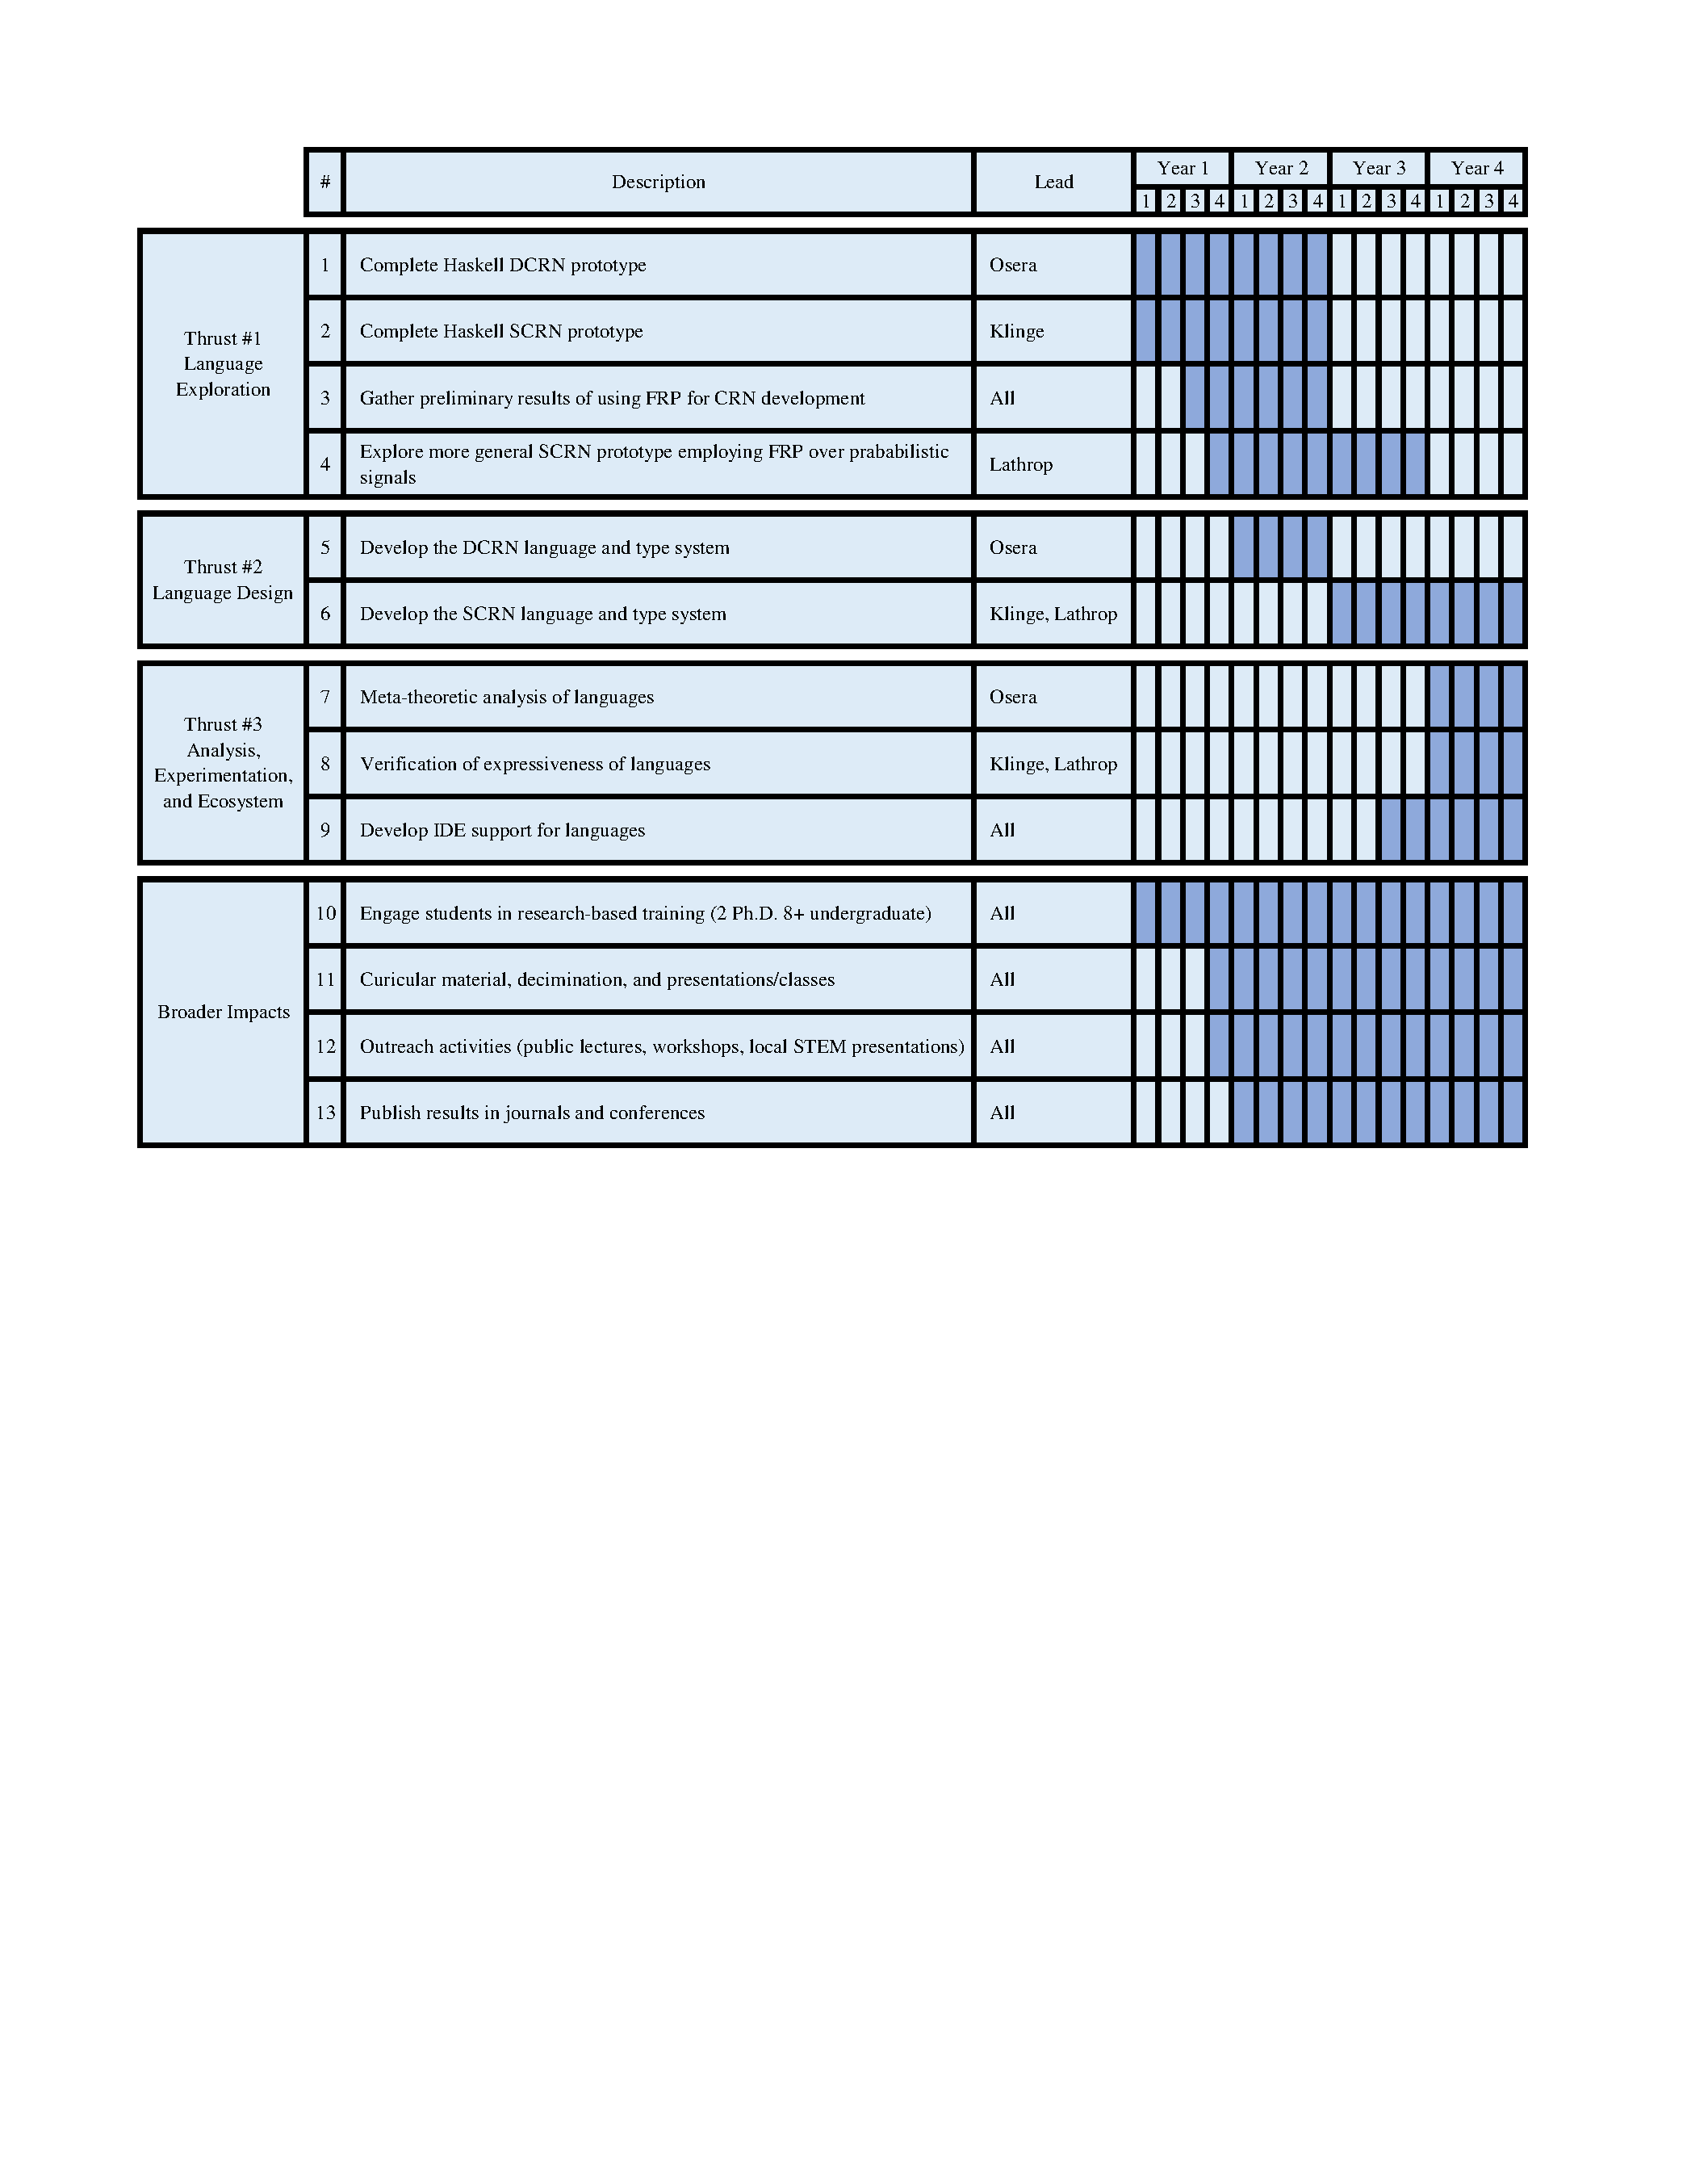
\includegraphics[width=6.4in]{TimeLine.pdf}
     \caption{Project Timeline}
 \end{figure}



    %!TEX root = project_description.tex

\section{Results from Prior NSF Support}

{\bf J. Lathrop} is a Co-PI on the current award CNS 1545028, CPS:Synergy: Safety-Aware Cyber-Molecular Systems, 10/15/2015 -- 8/31/2020, \$823,930.

\subsection*{Intellectual Merit}
The project combines methods from computer science and software engineering with methods from molecular biology to gain insights into how to develop cyber-molecular systems that are safe for use in dynamic and only partially understood environments.
The project has developed a refined formulation of what robustness means in deterministic chemical reaction networks. to  perform correctly even when crucial physical parameters are perturbed by small amounts and shown that nondeterministic finite automata can be simulated by deterministic chemical reaction networks that are provably robust in this sense.  
The project found that the use of advanced requirements engineering techniques for cyber-molecular systems enabled earlier removal of obstacles to safe operations.  Key results from the project also include the development of chemical reaction network models for standard safety building blocks needed for cyber-molecular systems \cite{oKlLaLu15,  cElLaLu17, cElKlLa17, jEKLLLM17}.
The project also implemented and evaluated in the laboratory a DNA origami-based reconfigurable nanosystem with potential as a force/energy diagnostic tool \cite{jMatHen16, oMath16}.    Publications describing these and additional results include \cite{cKlin16,  cHuaStu16, jCaLuSt18, cElKlLa17,  jHKLLL18}.        

\subsection*{Broader Impacts}
Eight Ph.D. students have been supported or partially supported by this award. Five of these have graduated since 2016:  Samuel Ellis co-advised by J. Lathrop and R. Lutz (Ph.D. 2017, now a Software Scientist at the NSF-funded Molecular Sciences Software Institute), Titus Klinge advised by J Lathrop and J Lutz  (Ph.D. 2016, now an Assistant Professor at Drake University, and prior appointments as Visiting Assistant Professor at Grinnell College and Carleton College), Adam Case advised by J. Lutz (Ph.D. 2016, now an Assistant Professor at Drake University), Don Stull advised J. Lutz (Ph.D. 2017, now a Lecturer at Iowa State University, and prior appointment at INRIA), Divita Mathur advised by E. Henderson (Molecular Biology Department) and J. Lutz (Ph.D. 2016, now at the U.S> Navel Research Laboratory).  Four Ph.D. students currently work in the Laboratory for Molecular Programming (LAMP).  

The project's REU supported research by two outstanding students, Gabrielle Ortman (graduated 2017)  and Chase Koehler (graduated 2018; co-authored a paper \cite{cKMHL18}).

J. Lutz developed  an undergraduate/graduate course on molecular programming and has taught it seven times with help from J. Lathrop, who taught it an eighth time in Fall, 2018.  As part of our educational outreach, J. Lathrop, J. Lutz and R. Lutz mentor students on molecular programming projects at two local undergraduate institutions, Grinnell College and Simpson College.
The investigators gave three tutorials on cyber-molecular systems at conferences (ASE 2015, ICSE 2016, RE 2018); a workshop at Simpson College and two invited keynotes (RE 2016, SAFECOMP 2018).
R. Lutz also gave the invited, public Dean's 2017 Spring Lecture at Iowa State University. \\

\noindent{\bf P.M. Osera} was the PI on award CCF 1651817, EAGER: Semi-Automated Type-Directed Programming, 2016--2019, \$159,991.
%
\subsection*{Intellectual Merit}
This project investigated the foundations of type-directed program synthesis along two dimensions: (1) extending the foundations to handle advanced typing features such as polymorphism and generalized algebraic datatypes and (2) realizing the foundations in a semi-automated program synthesis tool, \textsc{Scythe}, that supports type-directed programming in the Haskell programming language.

\subsection*{Broader Impacts}
This project supported 12 undergraduates for summer research opportunities over its lifetime.
Three of the alumni from this project are either in or applying to doctoral programs in computer science and/or mathematics.
The project also funded their travel to present their work at Midwest PL Summit as well as attend the Programming Languages Mentoring Workshop at PLDI and ICFP.

    % %!TEX root = project_description.tex

\section{Temporary Place for CRN Examples}
\todo{Remove this section once it isn't needed (or move it elsewhere).}
This section is for generating motivating molecular programming examples that relate to this project.
(So this section will eventually need to be removed.)

\subsection{Hailstone Function}
Suppose we'd like to create a stochastic CRN that, given \( n \) initial molecules of type \( X \), will eventually produce \( H(n) \) molecules of type \( Y \) where \( H(n) \) is the Hailstone function:
\begin{equation}
    H(n) = \begin{cases}
        n/2, &\text{ if }n\text{ is even}\\
        3n+1, &\text{ if }n\text{ is odd}
    \end{cases}
\end{equation}
Computing this function with an SCRN can be broken into the following parts: (1) checking if \( n \) is divisible by two, (2) dividing \( n \) by two, (3) multiplying \( n \) by three, (4) incrementing a value by 1, and (5) multiplexing the output so that either \( n/2 \) or \( 3n+1 \) output depending on the result of the parity check.
Below is the SCRN that successfully computes this function:
\begin{align}
    X &\goesto{} A_\text{odd} + B + C + D\label{eq:hailstone_split}\\
    A_\text{odd} + A_\text{odd} &\goesto{} A_\text{even}\label{eq:hailstone_parity1}\\
    A_\text{even} + A_\text{even} &\goesto{} A_\text{even}\label{eq:hailstone_parity2}\\
    A_\text{odd} + A_\text{even} &\goesto{} A_\text{odd}\label{eq:hailstone_parity3}\\
    2 B &\goesto{} Y_1\label{eq:halstone_n2}\\
    C &\goesto{} 3Y_2\label{eq:halstone_3n}\\
    A_\text{even} + Y_1 &\goesto{} A_\text{even} + Y + \widehat{Y}_1\label{eq:halstone_mux1}\\
    A_\text{odd} + Y_2 &\goesto{} A_\text{odd} + Y + \widehat{Y}_2\label{eq:halstone_mux2}\\
    A_\text{odd} + Y + \widehat{Y}_1 &\goesto{} A_\text{odd} + Y_1\label{eq:halstone_rev1}\\
    A_\text{even} + Y + \widehat{Y}_2 &\goesto{} A_\text{even} + Y_2\label{eq:halstone_rev2}\\
    2 D &\goesto{} D\label{eq:halstone_1}\\
    D + \widehat{D} &\goesto{} D\\
    2Y + 2\widehat{D} &\goesto{} Y + \widehat{D}\\
    A_\text{odd} + D &\goesto{} A_\text{odd} + Y + \widehat{D}\\
    A_\text{even} + Y + \widehat{D} &\goesto{} A_\text{even} + D\label{eq:halstone_1end}
\end{align}
In the above SCRN, reaction~\eqref{eq:hailstone_split} simply copies the number of \( X \)'s into four species that can be used to compute all four components necessary to finish the algorithm in parallel.
Reactions~\eqref{eq:hailstone_parity1}--\eqref{eq:hailstone_parity3} compute the Boolean parity function: if \( n \) is even, then the number of \( A_\text{even} \)'s converges to 1 and the number of \( A_\text{odd} \)'s converges to 0; likewise, if \( n \) is odd, then \( A_\text{odd} \) goes to 1 and \( A_\text{even} \) goes to 0.
Reaction~\eqref{eq:halstone_n2} computes \( n/2 \) and stores the answer in \( Y_1 \).
Reaction~\eqref{eq:halstone_3n} computes \( 3n \) and stores the answer in \( Y_2 \).
Reactions~\eqref{eq:halstone_mux1}--\eqref{eq:halstone_mux2} uses the result of the parity check and copies \( Y_1 \) into \( Y \) if \( A_\text{even} \) exists and \( Y_2 \) is copied if \( A_\text{odd} \) exists.
These multiplexer reactions can be reversed using reactions~\eqref{eq:halstone_rev1}--\eqref{eq:halstone_rev2} so that any values copied over prematurely can be undone once the parity computation finishes.
Finally, reactions~\eqref{eq:halstone_1}--\eqref{eq:halstone_1end} are responsible for computing the number 1 and copying it into \( Y \) if \( n \) is odd.

\subsection{Maximum Function}
There has been some recent research on \emph{composable} SCRNs, \ie, SCRNs that can be modularly combined with provably no problems occurring~\cite{doty19}.
It is well-known that these SCRNs must be \emph{output-oblivious}, \ie, the number of output molecules must be generated in a monotonically increasing fashion.
It is also well-known that computing the \emph{maximum} of two numbers cannot be computed by an SCRN in an output-oblivious fashion.

For example, below is an implementation of maximum with an SCRN:
\begin{align}
    X_1 &\goesto{} A_1 + Y\\
    X_2 &\goesto{} A_2 + Y\\
    A_1 + A_2 &\goesto{} B\\
    Y + B &\goesto{} \emptyset
\end{align}
The idea behind the above solution is that we can write the maximum of two numbers \( n_1, n_2 \) as:
\[
    \text{max}(n_1, n_2) = n_1 + n_2 - \text{min}(n_1, n_2).
\]
We compute the maximum function in this way by first computing the sum of \( X_1 \) and \( X_2 \) and storing the result in \( Y \), and then later subtracting from \( Y \) the minimum of \( X_1 \) and \( X_2 \) (this is computed with the \( A_1 + A_2 \goesto{} B \) reaction.)

Notice that this is NOT computing \( Y \) in a monotonically increasing fashion.
We first compute the sum (which could overshoot the maximum by quite a lot), and later we will decrease the total number of \( Y \)'s using the \( Y + B \goesto{} \emptyset \) reaction.

\subsection{Signal Multiplexer}
CRNs don't need to be considered machines that take in natural numbers and output natural numbers.
In fact, they are more naturally a \emph{signal processor} and can receive streams of molecules, \ie, a time-varying signal of molecules, and output a time-varying signal of molecules in response.

As a simple case of this, consider a deterministic CRN implementation of a multiplexer that receives two signals as input through species \( X_1 \) and \( X_2 \) along with a switch molecule \( S \).
If \( S \) is close to 1, then we want to have the output \( Y \) be identical to the signal provided through \( X_1 \), and if \( S \) is close to 0, then we want to have \( Y \) be identical to the signal \( X_2 \).
This cannot be done with perfect accuracy, but here is an approach:
\begin{align}
    S + X_1 &\goesto{k} S + X_1 + Y\\
    \overline{S} + X_2 &\goesto{k} \overline{S} + X_2 + Y\\
    Y &\goesto{k} \emptyset.
\end{align}
This approximates what we want because the ODE for \( Y \) is:
\begin{equation}
    \frac{dy}{dt} = k\left[s(t)x_1(t) + \overline{s}(t)x_2(t) - y(t)\right].
\end{equation}
Now, if \( s(t) + \overline{s}(t) = 1 \) for all \( t\in[0,\infty) \), then when \( S \) is close to 1, then \( \overline{S} \) is close to 0 and vice versa.
Thus, the above equation is really equal to one of the following:
\begin{align}
    \frac{dy}{dt} = k\left[x_1(t) - y(t)\right]\\
    \frac{dy}{dt} = k\left[x_2(t) - y(t)\right]
\end{align}
Thus, if \( S \) is high, then \( Y \) is ``chasing'' the concentration of \( X_1 \), and if \( S \) is low, then \( Y \) is ``chasing'' \( X_2 \).
If \( k \) is sufficiently large, then \( Y \) is a great approximation of the multiplexer we desire.

The technique of splitting the signal \( S \) into two is called \textbf{dual-rail representation} which allows us to use the presence of \( \overline{S} \) to have the same meaning as the absence of \( S \).

\subsection{Use of an LTL-like Temporal Logic}
Many of the above examples have a \emph{specification} or \emph{requirement} that can easily be written in an LTL like language.
For example, the hailstone requirement would simply be the following:
\begin{equation}\label{eq:hailstone_ltl}
    \Diamond\Box\left[y = H(x(0))\right].
\end{equation}
Recall that \( \Diamond\Phi \) is the ``future'' operator and means that eventually \( \Phi \) becomes true and that \( \Box\Psi \) is the ``globally'' operator and means that \( \Psi \) must always be true.
Therefore, equation~\eqref{eq:hailstone_ltl} means: ``eventually the number of \( Y \)'s will be equal to \( H(x_0) \) forever,'' which is exactly what we want.

Similarly, the maximum function can be written in an LTL-like language like this:
\begin{equation}\label{eq:max_ltl}
    \Diamond\Box[y=\max(x_1(0),x_2(0))]
\end{equation}

One thing that should be noted, is that most interesting SCRNs only \emph{probabilistically} converge to the correct answer.
SCRNs can only compute the semi-linear functions with probability 1, but they are Turing universal if you allow for any \( \epsilon > 0 \) probability of failure.
Therefore, to quantify most SCRN requirements, such as computing \( 2^n \), the requirement would need to be specified probabilistically such as:
\begin{equation}
    \mathcal{P}_{\ge1-\epsilon}\Diamond\Box[y=2^{x(0)}]
\end{equation}
which says that with probability \( 1 - \epsilon \) the LTL formula must be true.

There are probabilistic logics that exist, such as \emph{probabalistic computational tree logic} (\emph{PCTL}) and \emph{continuous stochastic logic} (\emph{CSL}), however, these formulae are \emph{state} formulae instead of \emph{path} formulae like LTL.
Therefore, we expect using a probabilistic version LTL will be more useful.

For DCRNs, there is a temporal logical called \emph{signal temporal logic} which is a continuous-time, continuous-space, variant of LTL.
It specifies precise relationships between the input signals and output signals.
For example, we might write an STL formula for the DCRN signal processor specification mentioned above with:
\begin{equation}
    \Box[(s=1)\implies(y=x_1)]\land\Box[(s=0)\implies(y=x_2)],
\end{equation}
which means that globally, if \( s(t)=1 \) then the concentration of \( y(t) \) is equal to \( x_1(t) \), and similarly if \( s(t) = 1 \), then the concentration of \( y(t) \) is equal to \( x_2(t) \).
This is a VERY strict requirement because \( Y \) must \emph{exactly} equal the corresponding concentration of the input.
(It is easy to prove this is impossible for DCRNs.)
Thus, it would be better if we had a way of \emph{approximately} satisfying an STL formula.
For example, if we look at the solution to the system of ODEs that corresponds to the DCRN given, what we really want is to compute a \emph{distance measure} of how close we are to satisfying the STL formula and then say we \emph{\(\epsilon\)}-approximately satisfy it if the measure is within \emph{\(\epsilon\)}.

We have other previous results that use continuous stochastic logic (CSL) to specify requirements and then \emph{formally verify} their correctness in model checkers like PRISM.
In particular, these papers:~\cite{cEHKLLL14,tosem19}.
We specify the high-level requirements of a ``watchdog timer'' in CSL, refine them into smaller requirements, prove that the sub-goals imply the super-goals, and then use PRISM to verify the leaf goals of the requirements tree.


    % %\setcounter{page}{1}
    % \bibliographystyle{abbrv}
    % \bibliography{../preface/master}
    {\setbox0\vbox{\bibliography{../preface/master}}}

\end{document}
